\documentclass{standalone}
\usepackage{tikz}
\usetikzlibrary{patterns, positioning}

\begin{document}
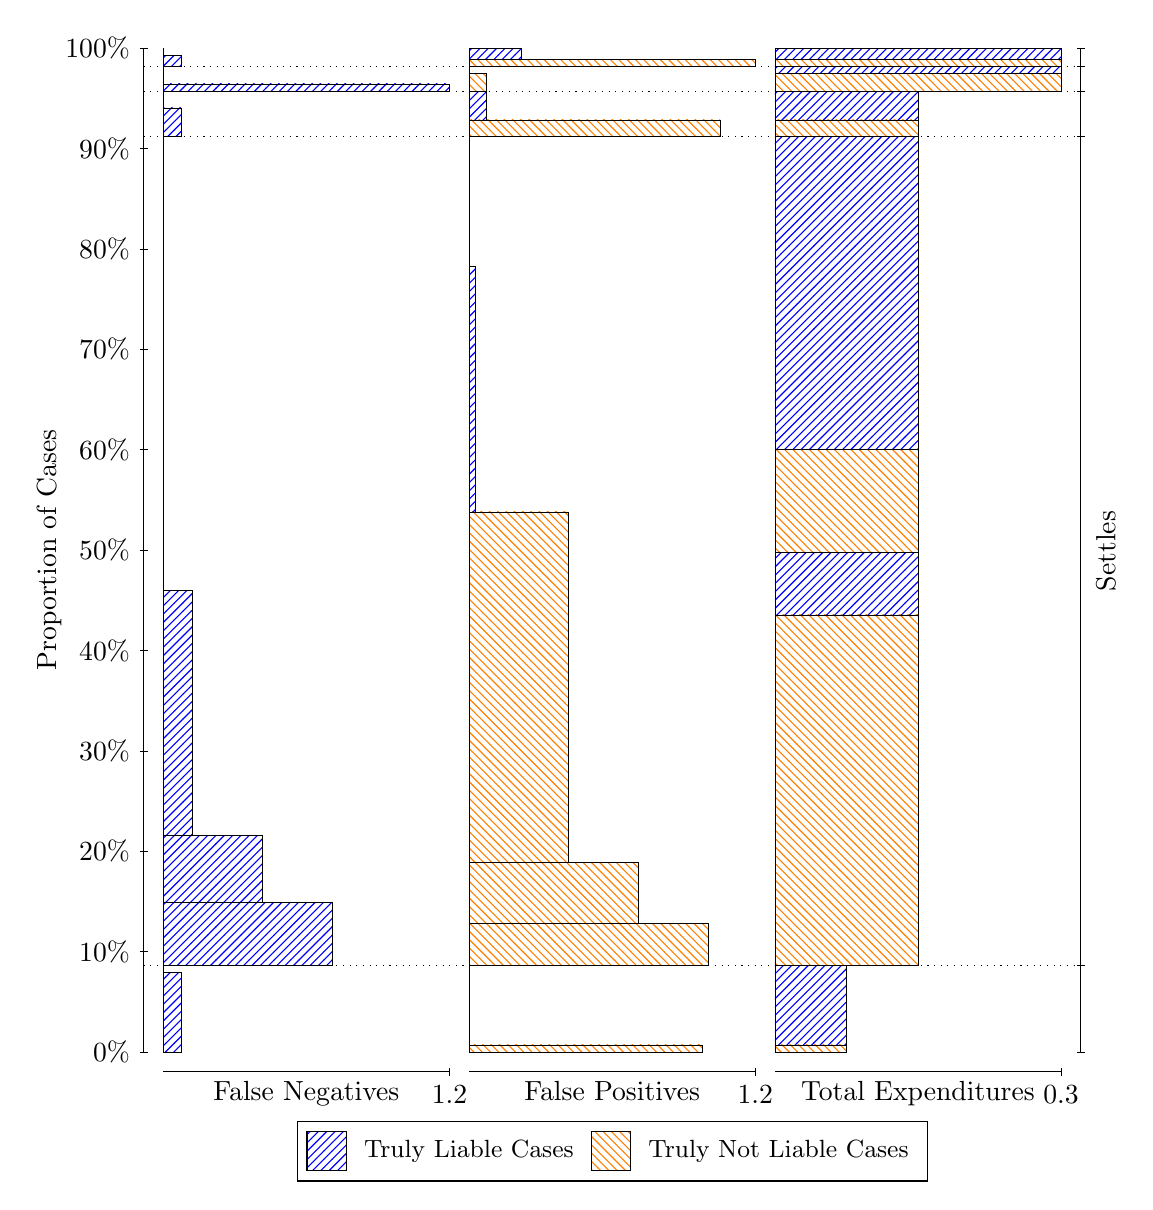
\begin{tikzpicture}
\draw[black, very thin] (1.5,1.75) -- (1.5,14.5);
\node[rotate=90, anchor=center] at (0.3, 8.125) {Proportion of Cases};
\draw[black, very thin] (1.45,1.75) -- (1.55,1.75);
\node[anchor=east] at (1.45, 1.75) {0\%};
\draw[black, very thin] (1.45,3.025) -- (1.55,3.025);
\node[anchor=east] at (1.45, 3.025) {10\%};
\draw[black, very thin] (1.45,4.3) -- (1.55,4.3);
\node[anchor=east] at (1.45, 4.3) {20\%};
\draw[black, very thin] (1.45,5.575) -- (1.55,5.575);
\node[anchor=east] at (1.45, 5.575) {30\%};
\draw[black, very thin] (1.45,6.85) -- (1.55,6.85);
\node[anchor=east] at (1.45, 6.85) {40\%};
\draw[black, very thin] (1.45,8.125) -- (1.55,8.125);
\node[anchor=east] at (1.45, 8.125) {50\%};
\draw[black, very thin] (1.45,9.4) -- (1.55,9.4);
\node[anchor=east] at (1.45, 9.4) {60\%};
\draw[black, very thin] (1.45,10.675) -- (1.55,10.675);
\node[anchor=east] at (1.45, 10.675) {70\%};
\draw[black, very thin] (1.45,11.95) -- (1.55,11.95);
\node[anchor=east] at (1.45, 11.95) {80\%};
\draw[black, very thin] (1.45,13.225) -- (1.55,13.225);
\node[anchor=east] at (1.45, 13.225) {90\%};
\draw[black, very thin] (1.45,14.5) -- (1.55,14.5);
\node[anchor=east] at (1.45, 14.5) {100\%};

\draw[black, very thin] (13.4,1.75) -- (13.4,14.5);
\draw[black, very thin] (13.35,1.75) -- (13.45,1.75);
\node[anchor=west] at (13.35, 1.75) {};
\draw[black, very thin] (13.35,2.8497) -- (13.45,2.8497);
\node[anchor=west] at (13.35, 2.8497) {};
\draw[black, very thin] (13.35,13.374) -- (13.45,13.374);
\node[anchor=west] at (13.35, 13.374) {};
\draw[black, very thin] (13.35,13.952) -- (13.45,13.952);
\node[anchor=west] at (13.35, 13.952) {};
\draw[black, very thin] (13.35,14.267) -- (13.45,14.267);
\node[anchor=west] at (13.35, 14.267) {};
\draw[black, very thin] (13.35,14.5) -- (13.45,14.5);
\node[anchor=west] at (13.35, 14.5) {};

\draw[black, very thin, pattern color=blue, pattern=north east lines] (1.75,1.75) rectangle (1.9724,2.7607);
\draw[black, very thin, pattern color=orange, pattern=north west lines] (1.75,2.7607) rectangle (1.75,2.8497);
\draw[black, very thin, pattern color=blue, pattern=north east lines] (1.75,2.8497) rectangle (3.9003,3.6469);
\draw[black, very thin, pattern color=blue, pattern=north east lines] (1.75,3.6469) rectangle (3.0105,4.5012);
\draw[black, very thin, pattern color=blue, pattern=north east lines] (1.75,4.5012) rectangle (2.1207,7.6159);
\draw[black, very thin, pattern color=orange, pattern=north west lines] (1.75,7.6159) rectangle (1.75,13.374);
\draw[black, very thin, pattern color=blue, pattern=north east lines] (1.75,13.374) rectangle (1.9724,13.74);
\draw[black, very thin, pattern color=orange, pattern=north west lines] (1.75,13.74) rectangle (1.75,13.952);
\draw[black, very thin, pattern color=blue, pattern=north east lines] (1.75,13.952) rectangle (5.3833,14.044);
\draw[black, very thin, pattern color=orange, pattern=north west lines] (1.75,14.044) rectangle (1.75,14.267);
\draw[black, very thin, pattern color=blue, pattern=north east lines] (1.75,14.267) rectangle (1.9724,14.407);
\draw[black, very thin, pattern color=orange, pattern=north west lines] (1.75,14.407) rectangle (1.75,14.5);
\draw[black, very thin, pattern color=orange, pattern=north west lines] (5.6333,1.75) rectangle (8.5993,1.839);
\draw[black, very thin, pattern color=blue, pattern=north east lines] (5.6333,1.839) rectangle (5.6333,2.8497);
\draw[black, very thin, pattern color=orange, pattern=north west lines] (5.6333,2.8497) rectangle (8.6735,3.388);
\draw[black, very thin, pattern color=orange, pattern=north west lines] (5.6333,3.388) rectangle (7.7837,4.1559);
\draw[black, very thin, pattern color=orange, pattern=north west lines] (5.6333,4.1559) rectangle (6.8939,8.6081);
\draw[black, very thin, pattern color=blue, pattern=north east lines] (5.6333,8.6081) rectangle (5.7075,11.723);
\draw[black, very thin, pattern color=blue, pattern=north east lines] (5.6333,11.723) rectangle (5.6333,13.374);
\draw[black, very thin, pattern color=orange, pattern=north west lines] (5.6333,13.374) rectangle (8.8218,13.586);
\draw[black, very thin, pattern color=blue, pattern=north east lines] (5.6333,13.586) rectangle (5.8558,13.952);
\draw[black, very thin, pattern color=orange, pattern=north west lines] (5.6333,13.952) rectangle (5.8558,14.175);
\draw[black, very thin, pattern color=blue, pattern=north east lines] (5.6333,14.175) rectangle (5.6333,14.267);
\draw[black, very thin, pattern color=orange, pattern=north west lines] (5.6333,14.267) rectangle (9.2667,14.36);
\draw[black, very thin, pattern color=blue, pattern=north east lines] (5.6333,14.36) rectangle (6.3007,14.5);
\draw[black, very thin, pattern color=orange, pattern=north west lines] (9.5167,1.75) rectangle (10.425,1.839);
\draw[black, very thin, pattern color=blue, pattern=north east lines] (9.5167,1.839) rectangle (10.425,2.8497);
\draw[black, very thin, pattern color=orange, pattern=north west lines] (9.5167,2.8497) rectangle (11.333,7.3019);
\draw[black, very thin, pattern color=blue, pattern=north east lines] (9.5167,7.3019) rectangle (11.333,8.099);
\draw[black, very thin, pattern color=orange, pattern=north west lines] (9.5167,8.099) rectangle (11.333,9.4052);
\draw[black, very thin, pattern color=blue, pattern=north east lines] (9.5167,9.4052) rectangle (11.333,13.374);
\draw[black, very thin, pattern color=orange, pattern=north west lines] (9.5167,13.374) rectangle (11.333,13.586);
\draw[black, very thin, pattern color=blue, pattern=north east lines] (9.5167,13.586) rectangle (11.333,13.952);
\draw[black, very thin, pattern color=orange, pattern=north west lines] (9.5167,13.952) rectangle (13.15,14.175);
\draw[black, very thin, pattern color=blue, pattern=north east lines] (9.5167,14.175) rectangle (13.15,14.267);
\draw[black, very thin, pattern color=orange, pattern=north west lines] (9.5167,14.267) rectangle (13.15,14.36);
\draw[black, very thin, pattern color=blue, pattern=north east lines] (9.5167,14.36) rectangle (13.15,14.5);
\draw[black, dotted] (1.5,2.8497) -- (13.4,2.8497);
\draw[black, dotted] (1.5,13.374) -- (13.4,13.374);
\draw[black, dotted] (1.5,13.952) -- (13.4,13.952);
\draw[black, dotted] (1.5,14.267) -- (13.4,14.267);
\draw[black, very thin] (1.75,1.5) -- (5.3833,1.5);
\node[anchor=north] at (3.5667, 1.5) {False Negatives};
\draw[black, very thin] (5.3833,1.45) -- (5.3833,1.55);
\node[anchor=north] at (5.3833, 1.45) {1.2};

\draw[black, very thin] (5.6333,1.5) -- (9.2667,1.5);
\node[anchor=north] at (7.45, 1.5) {False Positives};
\draw[black, very thin] (9.2667,1.45) -- (9.2667,1.55);
\node[anchor=north] at (9.2667, 1.45) {1.2};

\draw[black, very thin] (9.5167,1.5) -- (13.15,1.5);
\node[anchor=north] at (11.333, 1.5) {Total Expenditures};
\draw[black, very thin] (13.15,1.45) -- (13.15,1.55);
\node[anchor=north] at (13.15, 1.45) {0.3};


\node[black, centered, rotate=90] at (13.72, 8.112) {Settles};




\draw (7.449999999999999,1.5) node[draw=none] (baseCoordinate) {};
\begin{scope}[align=center]
        \matrix[scale=0.5, draw=black, below=0.5cm of baseCoordinate, nodes={draw}, column sep=0.1cm]{
            \node[rectangle, draw, minimum width=0.5cm, minimum height=0.5cm, pattern=north east lines, pattern color=blue] {}; &
            \node[draw=none, font=\small] (B) {Truly Liable Cases}; &
            \node[rectangle, draw, minimum width=0.5cm, minimum height=0.5cm, pattern=north west lines, pattern color=orange] {}; &
            \node[draw=none, font=\small] (B) {Truly Not Liable Cases}; \\
            };
\end{scope}

\end{tikzpicture}
\end{document}